\documentclass{article}
\author{Andrea Casalino}
\title{Gaussian Mixture Models}

\RequirePackage[margin=2cm]{geometry}
\geometry{left=2cm,right=2cm,marginparwidth=6.8cm,marginparsep=1.5cm,top=1.5cm,bottom=1.5cm,footskip=2\baselineskip}

\usepackage[T1]{fontenc}
\usepackage[utf8]{inputenc}
\usepackage[default]{lato}
\usepackage{graphicx,color, import}
\usepackage{amssymb, amsmath}
%\usepackage{hyperref}
\usepackage{url}
\usepackage[]{algorithm2e}
\usepackage[toc,page]{appendix}

\begin{document}
\maketitle

\newpage
\section{What is a Gaussian Mixture model?}

A Gaussian Mixture Model (GMM) is a class of probability distribution functions, often adopted to approximate unknown distributions. 
GMM is basically a mixture (Section \ref{sec:mixture})of Gaussians (Section \ref{sec:Gauss}).
\\
The generic probability density function (aka pdf) $f$ of a continuous random variable $X$, having $\mathcal{X} \in \mathbb{R}^n$ as domain, is a function defined as follows:
 \begin{eqnarray}
f:\mathcal{X} \rightarrow [0,1] 
\\
\int_{\mathcal{X}} f(X) dx_1 \cdot \cdots \cdot dx_n = 1
\label{eq:pdf}
\end{eqnarray}  
Prior to discuss the GMM properties, the expectation $\mathbb{E}$ operator must be introduced.
The expectation $\mathbb{E}$ of a distribution $f$ w.r.t a function $g(X)$ defined over the same domain is equal to:
\begin{eqnarray}
\mathbb{E}_f[g(X)] =  \int_{\mathcal{X}} f(X)g(X) dx_{1,\cdots,n}
\end{eqnarray}

\section{Gaussian distributions}
\label{sec:Gauss}

Among all the possible distributions, Gaussians are ones of the most important. The mono-variate Gaussian distribution is a pdf defined as follows:
\begin{eqnarray}
\phi _{(\mu,\Sigma)}&:&\mathcal{X} \rightarrow [0,1] \\
\phi _{(\mu,\Sigma)}(x) &=& \frac{1}{\sqrt{2 \pi \Sigma }} exp \bigg( -\frac{1}{2} (x-\mu) \cdot \frac{1}{\Sigma} \cdot (x-\mu) \bigg)
\label{eq:Gauss_pdf}
\end{eqnarray}
where $X \subset \mathbb{R}$.
$\Sigma$ and $\mu$ are the covariance and mean of the distribution and are obtained through the following expectations:
\begin{eqnarray}
\mu &=& \mathbb{E}_{\phi}[x] = \int_{\mathcal{X}} \phi_{(\mu, \Sigma)}(x)x dx \\
\Sigma &=& \mathbb{E}_{\phi}[(x-\mu)^2] = \int_{\mathcal{X}} \phi_{(\mu, \Sigma)}(x-\mu)^2 dx
\end{eqnarray}
Figure \ref{fig:normal_mono} reports examples of Gaussian distributions.
\\
The multivariate version of a Gaussian is built generalizing the uni-variate one. Indeed, every multivariate Gaussian distribution can be seen, in a proper space, as a union of $n$ independent Gaussian distributions. Indeed, suppose to have $n$ independent Gaussians having a null means and the variances equal to $\Sigma_{1,\cdots,n}$.
They form a multivariate Gaussian distribution $\Phi_{(0, \Sigma)}$, with a covariance matrix $\Sigma$ equal to the following diagonal matrix:
\begin{eqnarray}
\Sigma = \begin{bmatrix}
\Sigma_1 &  & \\ 
 & \ddots & \\ 
 &  & \Sigma_n
\end{bmatrix}
\end{eqnarray} 
Since all the Gaussians are independent, the expression of the density function is obtained as the following product:
\begin{eqnarray}
\Phi_{(0, \Sigma)}(Y) &=& \phi_{(0,\Sigma_1)}(y_1) \cdot \cdots \cdot \phi_{(0,\Sigma_n)}(y_n) \\
\Phi_{(0, \Sigma)}(Y) &=&  \frac{1}{\sqrt{2 \pi \Sigma_1}} exp \bigg( -\frac{1}{2} \frac{y_1^2}{\Sigma_1}  \bigg) \cdot \cdots \cdot \frac{1}{\sqrt{2 \pi \Sigma_n}} exp \bigg( -\frac{1}{2} \frac{y_n^2}{\Sigma_n} \bigg) \\
\Phi_{(0, \Sigma)}(Y) &=& \frac{1}{\sqrt{ {(2 \pi)}^n \cdot \Sigma_1 \cdot \cdots \cdot \Sigma_n }  } exp \bigg( -\frac{1}{2} \sum_{i=1}^n \frac{y_i^2}{\Sigma_i}  \bigg) \\
\Phi_{(0, \Sigma)}(Y) &=& \frac{1}{\sqrt{ {(2 \pi)}^n \cdot \left | \Sigma \right | }  } exp \bigg( -\frac{1}{2} Y^T \begin{bmatrix}
\frac{1}{\Sigma_1} &  & \\ 
 & \ddots & \\ 
 &  & \frac{1}{\Sigma_n}
\end{bmatrix} Y \bigg) \\
\Phi_{(0, \Sigma)}(Y) &=& \frac{1}{\sqrt{ {(2 \pi)}^n \cdot \left | \Sigma \right | }  } exp \bigg( -\frac{1}{2} Y^T \Sigma^{-1} Y \bigg)
\end{eqnarray}
Notice that:
\begin{eqnarray}
\int_{\mathcal{Y}} \Phi_{(0, \Sigma)}(Y) dy_{1,\cdots,n} = 1
\end{eqnarray}
is ensured due to the fact that the following single integrals are all equal to 1 (equation (\ref{eq:Gauss_pdf})):
\begin{eqnarray}
\Phi_{(0, \Sigma)}(Y) = \bigg( \int_{\mathcal{Y}} \frac{1}{\sqrt{2 \pi \Sigma_1}} exp \bigg( -\frac{1}{2} \frac{y_1^2}{\Sigma_1}  \bigg) dy_1 \bigg) \cdot \cdots \cdot \bigg( \int_{\mathcal{Y}} \frac{1}{\sqrt{2 \pi \Sigma_n}} exp \bigg( -\frac{1}{2} \frac{y_n^2}{\Sigma_n}  \bigg) dy_1 \bigg)
\end{eqnarray}
Moreover it is true that the covariance matrix $\Sigma$ can be obtained through the following expectation:
\begin{eqnarray}
\Sigma = \mathbb{E}_{\Phi} [ Y \cdot Y^T ] = \int _{\mathcal{Y}} \Phi_{(0,\Sigma)}(Y) Y\cdot Y^T dy_{1,\cdots,n}
\end{eqnarray}
In the domain of $\mathcal{Y}$, the multivariate Gaussian $\Phi(Y)$ is made of many independent Gaussians. Anyway, when performing a change of variables, the same distribution becomes a general multivariate Gaussian, having the variables in the new domain that are correlated. Consider to set $Y=R \cdot X^{'}$, with $R$ that is a rotation matrix, i.e. $R^{-1} = R^T$.  $X^{'}$ is in turn described by a multivariate Gaussian having a density defined as follows:
\begin{eqnarray}
\Phi_{(0, \Sigma)}(X^{'}) &=& \frac{1}{\sqrt{ {(2 \pi)}^n \cdot \left | \Sigma \right | }  } exp \bigg( -\frac{1}{2} {X^{'}}^T R^T \Sigma^{-1} R X^{'} \bigg) \\
\Phi_{(0, \Sigma^{'})}(X^{'}) &=& \frac{1}{\sqrt{ {(2 \pi)}^n \cdot \left | \Sigma^{'} \right | }  } exp \bigg( -\frac{1}{2} {X^{'}}^T ({\Sigma^{'}})^{-1} X^{'} \bigg)
\end{eqnarray} 
The above simplifications are due to the fact that:
\begin{eqnarray}
\Sigma^{'} &=& R^T \Sigma R \\
({\Sigma^{'}})^{-1} &=& R^{-1} \Sigma^{-1} R = R^T \Sigma^{-1} R 
\end{eqnarray}
Moreover, since $R$ is a rotation matrix, $\Sigma^{'}$ is symmetric positive definite (since $\Sigma_{1,\cdots,n} \geq 0$). Additionally $\left | \Sigma \right | = \left | \Sigma^{'} \right |$. 
Applying an additional transformation of the form $X = X^{'} + \mu$, a distribution with a non zero mean (in the new domain) can be obtained. $X$ is the generic multivariate Gaussian, with a density equal to:
\begin{eqnarray}
\Phi_{(\mu, \Sigma^{'})}(X) = \frac{1}{\sqrt{ {(2 \pi)}^n \cdot \left | \Sigma^{'} \right | }  } exp \bigg( -\frac{1}{2} {(X - \mu)}^T ({\Sigma^{'}})^{-1} (X - \mu) \bigg)
\label{eq:Gauss_multi_pdf}
\end{eqnarray}
Indeed, applying a rotation and a translation, every multivariate Gaussian can be obtained from a simple set of independent uni-variate Gaussians. Section \ref{sec:sample} reports a way to compute in a precise way the change of variables to perform to obtain a Gaussian with a certain mean and covariance.
Figure \ref{fig:normal_change_frame} summarizes the above considerations.

\begin{figure}
	\centering
\begin{tabular}{ll}
\begin{minipage}[t]{0.45 \columnwidth}
	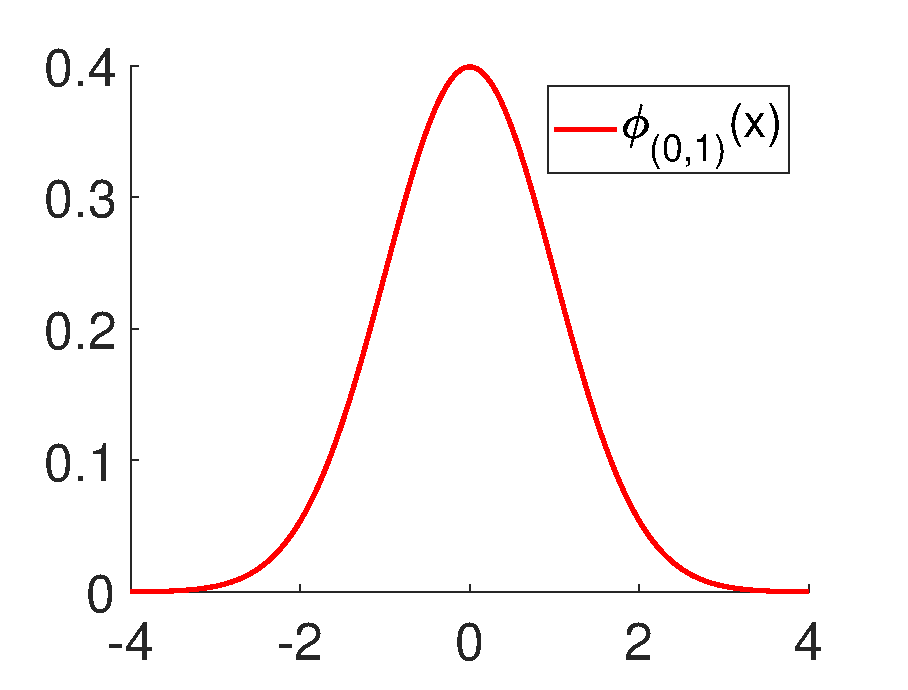
\includegraphics[width=0.8 \columnwidth]{./image/normal_01.eps}
\end{minipage}
 & 
\begin{minipage}[t]{0.45 \columnwidth}
	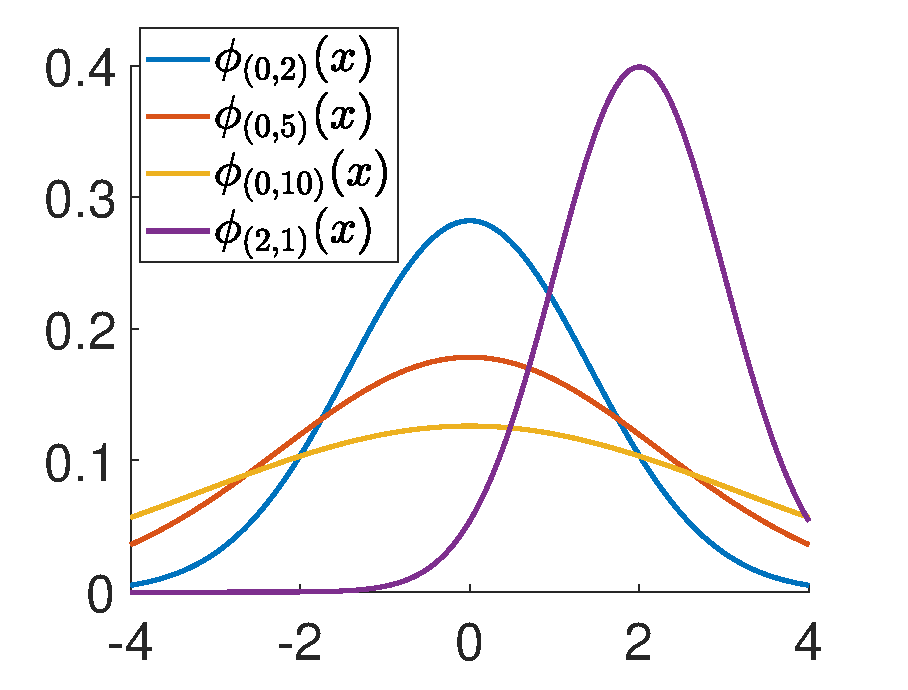
\includegraphics[width=0.8 \columnwidth]{./image/normal_02.eps}
\end{minipage}
\end{tabular}
\caption{On the left the uni-variate Gaussian distribution having a 0 mean and unitary variance, while on the right examples Gaussians having different values for the variance and the mean.}
	\label{fig:normal_mono}
\end{figure} 

\begin{figure}
	\centering
\begin{tabular}{ll}
\begin{minipage}[t]{0.55 \columnwidth}
	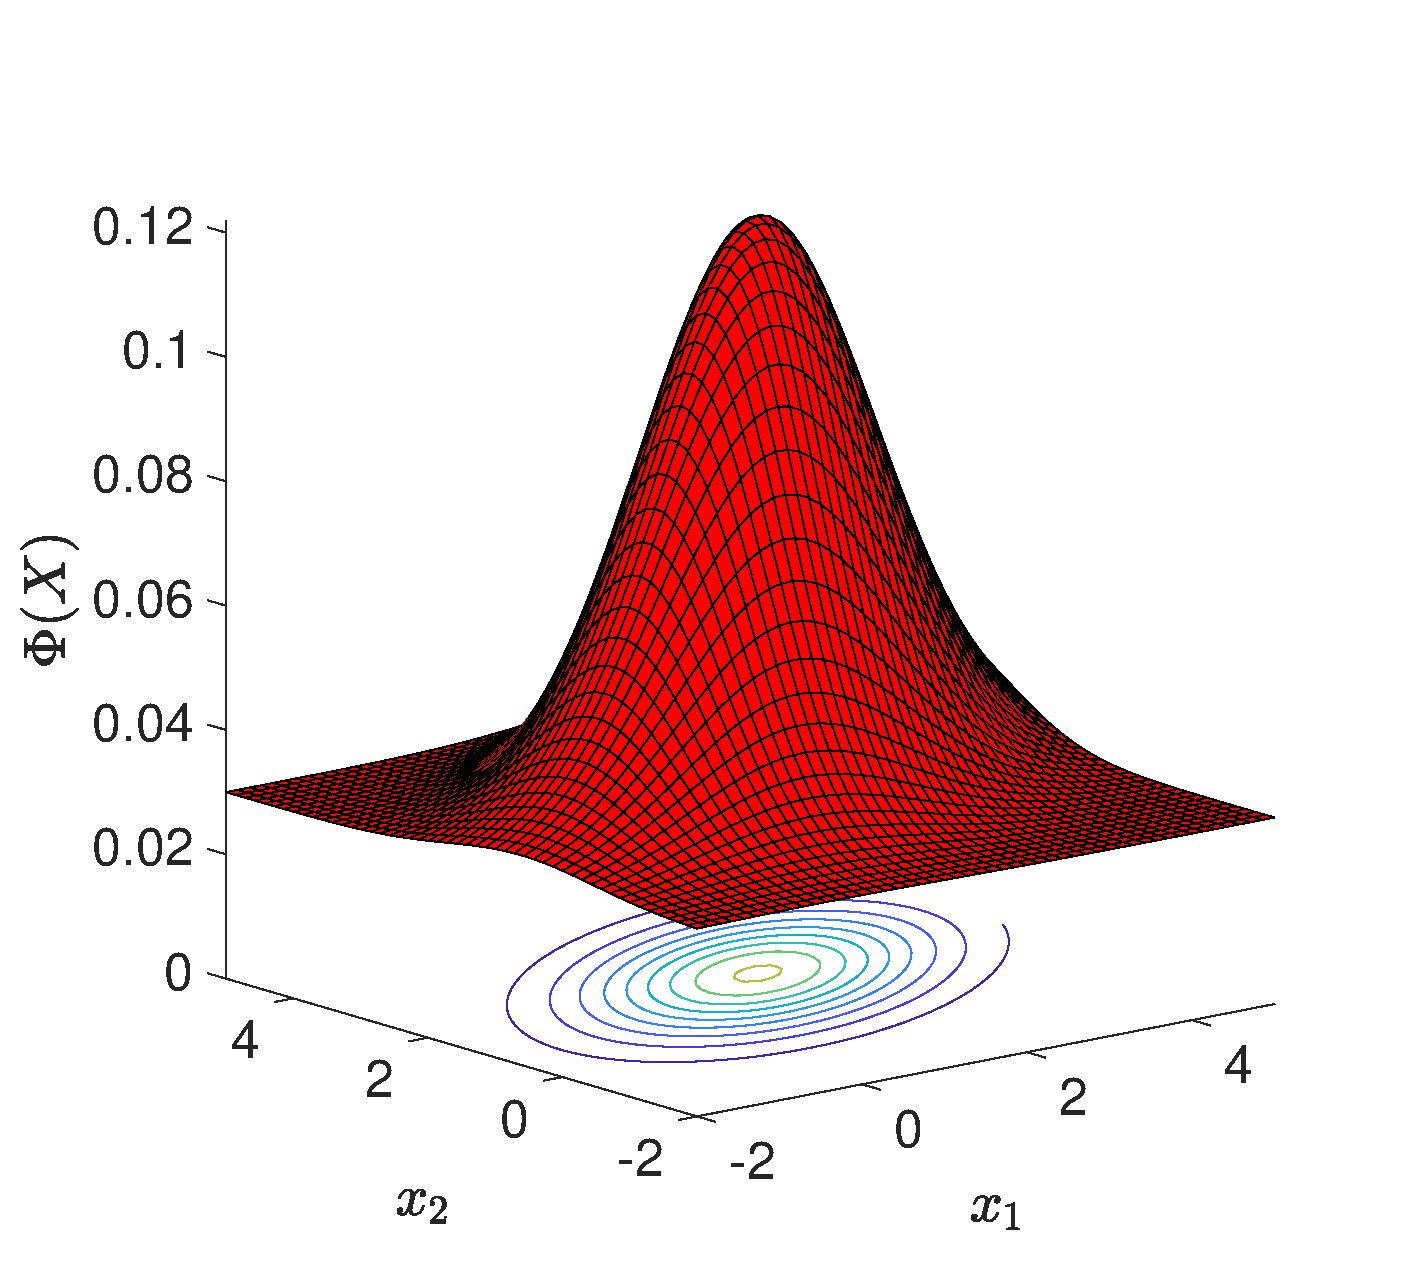
\includegraphics[width=0.8 \columnwidth]{./image/normal_04.eps}
\end{minipage}
 & 
\begin{minipage}[t]{0.4 \columnwidth}
\def\svgwidth{ \columnwidth}
\import{./image/}{normal_05.pdf_tex} 
\end{minipage}
\end{tabular}
\caption{Example of a bi-variate Gaussian. When considering $X \in \mathcal{X}$, $x_1$ and $x_2$ are correlated, while when passing in the space of $\mathcal{Y}$, the bi-variate Gaussian is simply a union of two independent mono-variate Gaussians. On the left the distribution $\Phi(X)$ is represented, together with its level curve (bottom of the figure). On the right, the transformation to apply for obtaining the space $\mathcal{Y}$.}
	\label{fig:normal_change_frame}
\end{figure}

\section{Mixture models}
\label{sec:mixture}

Mixture models are used to define a probability density function as the combination of a certain number of simpler ones.
It is possible to define a generic mixture model, by combining $N$ probability densities $f_{1,\cdots,N}$ satisfying equation (\ref{eq:pdf}) and sharing the same domain $\mathcal{X}$. Indeed, considering $N$ weights $\lambda _{1,\cdots,N}$, the density of the mixture $f_{mix}$ is defined as follows:
\begin{eqnarray}
f_{mix}(x) = \sum_{i=1}^{N} \lambda_{i} f_i(x)
\label{eq:mix_pdf}
\end{eqnarray}

To ensure that $f_{mix}$ is in turn a valid probability density function satisfying equation \ref{eq:pdf}, it is necessary to impose that the combination expressed in equation (\ref{eq:mix_pdf}) should be convex, meaning that:
\begin{eqnarray}
\sum_{i=1}^{N} \lambda_{i} = 1
\label{eq:sum_w_mix}
\end{eqnarray}
In fact, when the above specification holds, it is true that:
\begin{eqnarray}
\int_{X} f_{mix}(x) dx &=& \int_{X} [ \lambda_1 f_1(x) + \cdots + \lambda_N f_N(x) ] dx \nonumber\\
&=&  \int_{X}  \lambda_1 f_1(x) dx + \cdots + \int_{X} \lambda_N f_N(x) dx \nonumber\\
&=&   \lambda_1\int_{X} f_1(x) dx + \cdots + \lambda_N \int_{X} f_N(x) dx \nonumber\\
\int_{X} f_{mix}(x) dx &=&   \lambda_1 + \cdots + \lambda_N = \sum_{i=1}^{N} \lambda_{i} = 1
\end{eqnarray}
The simplifications made in the above equation are justified by the fact that every function $f_i$ is a probability distribution function satisfying equation (\ref{eq:pdf}):
\begin{eqnarray}
\left\{\begin{matrix}
\int_{X} f_1(x)dx = 1
\\ 
\vdots 
\\ 
\int_{X} f_N(x)dx = 1
\end{matrix}\right.
\end{eqnarray}

It is worth noticing that no particular hypothesis were posed about the combining distributions $f_{1,\cdots,N}$. We need only to require they are valid probability density functions defined over the same domain. The above considerations are true also when considering multivariate distributions.

\section{Gaussian Mixture models}

Gaussian mixture models are particular mixture models combining $N$ multivariate Gaussian distributions.
The distribution of a GMM, $f_{GMM}$, is defined in this way:
\begin{eqnarray}
f_{GMM}(x_{1,\cdots,n}) &=& \sum_{i=1}^{N} \lambda_i \Phi_{(\mu_i, \Sigma_i)}(x_{1,\cdots,n}) 
\end{eqnarray}
where in the above equation $\Sigma_i$ and $\mu_i$ are the variance and mean of the $i^{th}$ Gaussian distribution in the mixture. 
An example of uni-variate Gaussian mixture is reported in Figure \ref{fig:GMM_uni}.
\\
GMM can be also adopted for approximating complex unknown distributions.  Indeed, considering the proper number of clusters, any kind of probability distribution can be approximated by a GMM. 
\\
As an example, consider to approximate the uniform distribution $U(0,1)$ with a GMM, $f_{approx}$, made of $n_{mix}$ components defined as follows:
\begin{eqnarray}
f_{approx}(x | n_{mix}) &=& \sum _{i=1}^{n_{mix}}  \Phi_{(\mu_i, \Sigma_i)} \nonumber\\
\Sigma_i &=& \bigg( {\frac{1}{n_{mix}}} \bigg)^{2} \,\,\,\,\,\, 
\mu_i = \frac{1}{n_{mix}} \bigg( i - 0.5 \bigg)
\label{eq:GMM_pdf}
\end{eqnarray}
In Figure \ref{fig:f_approx}, the density of $U(0,1)$ is compared with the one of $f_{approx}$, varying the number of approximating clusters. As can be visually appreciated, the approximation error decreases when increasing the number of clusters in the model. This phenomenon is not always verified when considering other kind of distributions.

\begin{figure}
	\centering
	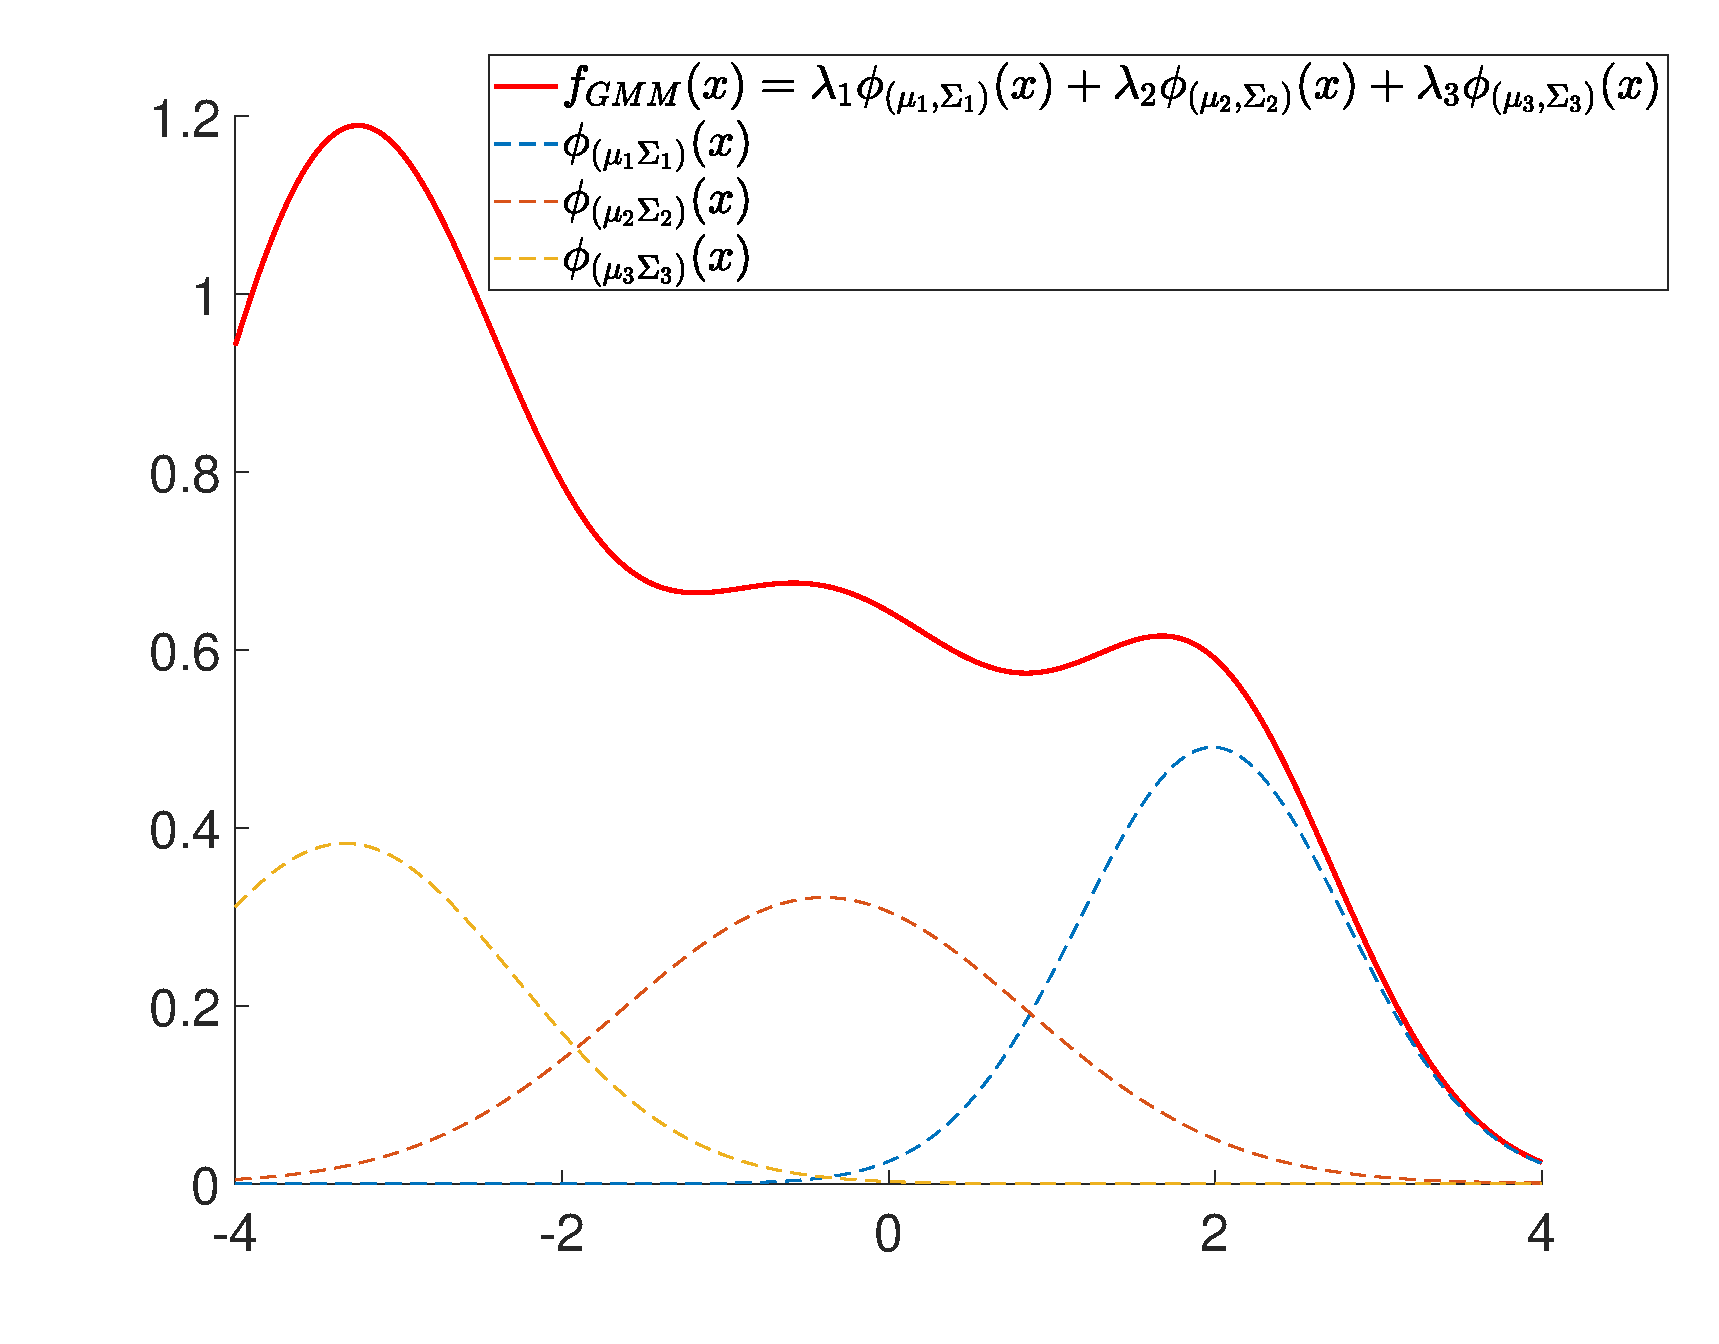
\includegraphics[width=0.6 \columnwidth]{./image/normal_03.eps}
	\caption{Example of Gaussian mixture involving univariate Gaussians. The parameters of the mixture have the same values: $\mu_1 =  1.9852, \mu_2 = -0.3957, \mu_3= -3.3294$; $\Sigma_1 =  0.8131, \Sigma_2 = 1.24, \Sigma_3= 1.0429$ and $\lambda_1 = 0.3, \lambda_2 = 0.6, \lambda_3 = 0.1$.}
	\label{fig:GMM_uni}
\end{figure} 

\begin{figure}
	\centering
	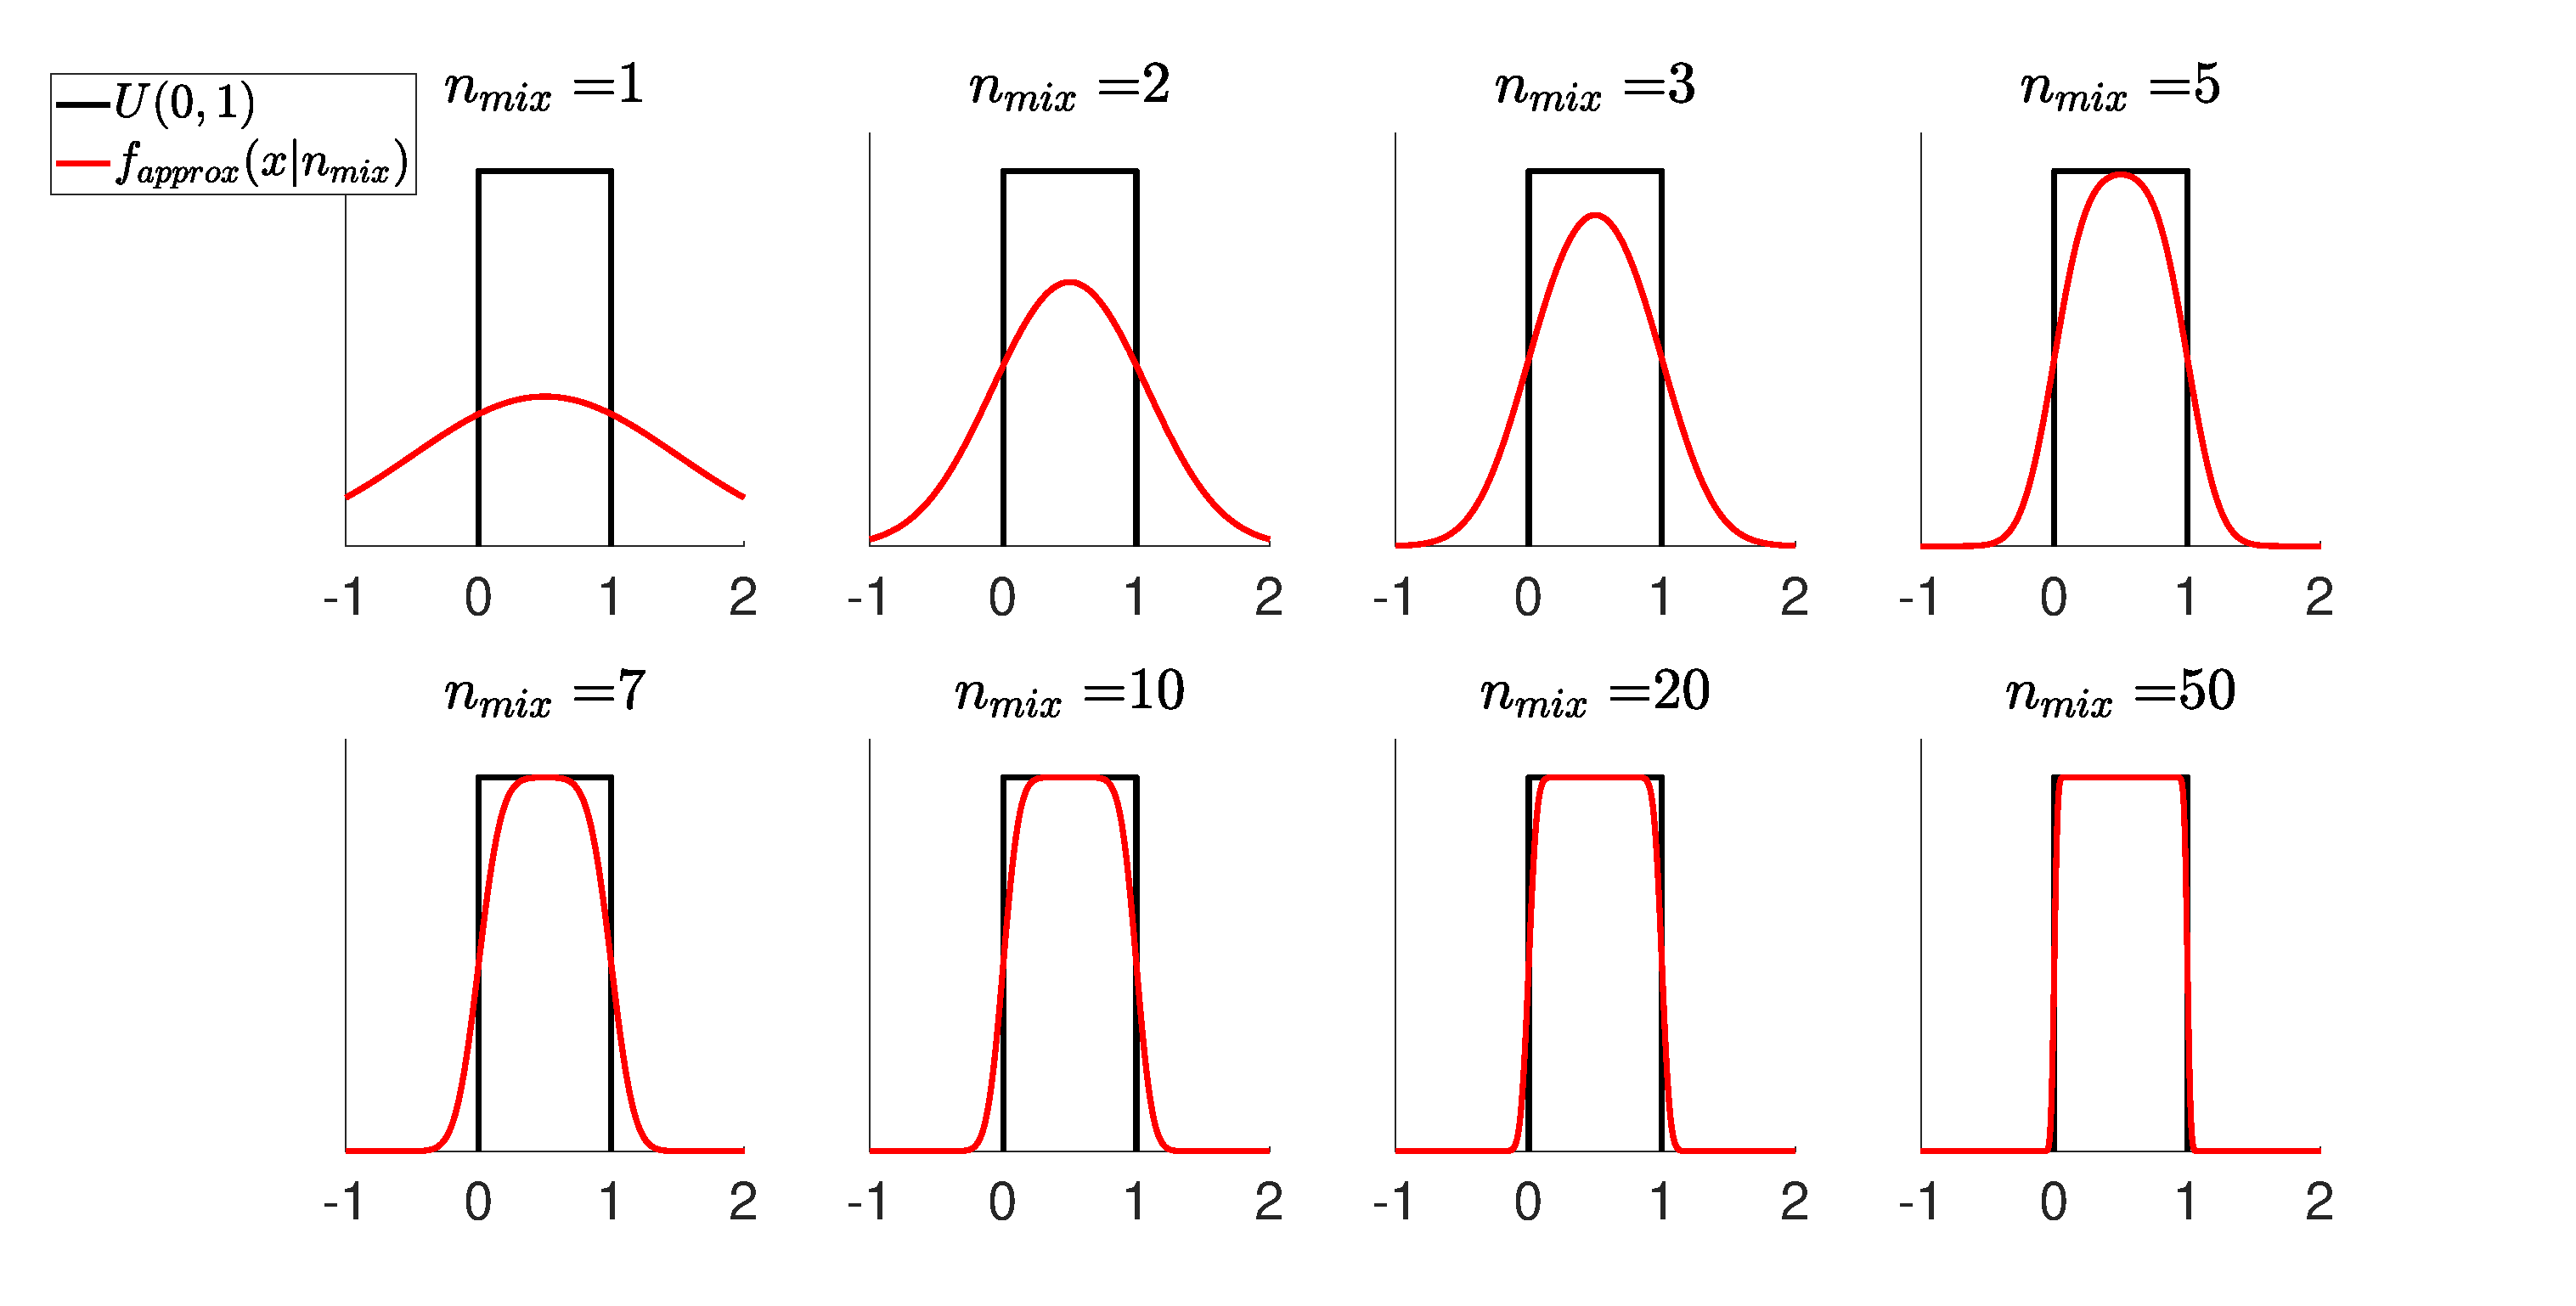
\includegraphics[width=0.99 \columnwidth]{./image/f_approx.eps}
	\caption{The uniform density between 0 and 1 is compared with an approximating mixture, varying the number of components.}
	\label{fig:f_approx}
\end{figure} 

\section{Learning of GMM using Expectation maximization}

The values of the weights $\lambda_{1,\cdots,N}$, as well the parameters characterizing every single density $\Phi_i$ in the mixture, i.e. the covariances and the means, are tuned through a learning process which considers as training set $S = \langle X^1, \cdots  , X^M \rangle$, \textit{i.e.} $M$ realizations of $f_{GMM}$. Such learning process is performed using the expectation maximization algorithm.
\\
EM, is essentially an iterative algorithm that starts from an initial guess for the parameters of the clusters $\theta = \lbrace \cdots \lambda_i, \Sigma_i, \mu_i, \cdots \rbrace$, and then adjusts the model values until the convergence to a maximum for the likelihood $L(\theta | S)$.
EM is considered as an unsupervised algorithm, since only the number of clusters must be specified when performing learning, i.e.how many clusters consider for the mixture, omitting the labels \footnote{The Gaussian in the mixture that produced that sample} of the elements in the training set.
\\
The expectation-maximization algorithm can be adopted not only to learn GMM.  It is in general used to learn the optimal parameter $\theta$ of a model having some observed variables $X_{1,\cdots,n}$ and also some latent ones $Z_{1,\cdots}$. $Z$ are variables whose values are hidden, but are linked in a probabilistic way to those observed, \textit{i.e.} $X$. 
Learning is done according to a training set $S = \langle X^1, \cdots , X^M \rangle$, made of realizations of $X$: the corresponding values for $Z^{1,\cdots,M}$ are not known.  
\\
EM starts from an initial guess $\theta_0$ and iteratively improves it.
At every iteration, an Expectation and a Maximization are preformed, explaining the name of the algorithm. The Expectation step is performed for taking into account the expectation of the likelihood w.r.t. $Z$, in order to maximise the likelihood of the training set, no matter the values for $Z$, which are, in a certain sense, eliminated.
\\
As usually done, learning aims at maximizing a likelihood function involving the training set. In this case, we would like to find those $\theta$ maximising $L(X|\theta)$ \footnote{For the moment assume to have a single sample $X$ in the training set, i.e. $S=\lbrace X \rbrace$ and $L(S|\theta) = L(X|\theta)$}. $L(X|\theta)$ can be computed considering how the joint conditioned distribution of $X,Z$ is factorizable: 
\begin{eqnarray}
\mathbb{P}(X,Z|\theta) &=& \mathbb{P}(Z|X,\theta) \mathbb{P}(X|\theta) \nonumber\\
\mathbb{P}(X|\theta) &=& \frac{\mathbb{P}(X,Z|\theta)}{\mathbb{P}(Z|X,\theta)} 
\end{eqnarray}
Passing to the logarithms we obtain:
\begin{eqnarray}
log(\mathbb{P}(X|\theta)) = log(\mathbb{P}(X,Z|\theta)) - 
log(\mathbb{P}(Z|X,\theta)) 
\label{eq:EM:log_EM_lkl}
\end{eqnarray}
We are now in position to describe the Expectation step of EM algorithm. Right hand side of equation (\ref{eq:EM:log_EM_lkl}) is a function of $Z$, which is unfortunately unknown. For this reason, we want to marginalize $Z$, by passing to the expectations w.r.t to density $\mathbb{P}(Z|X,\theta _k)$, where  $\theta _k$ are the values of the parameter at step $k$:
\begin{eqnarray}
\sum_{Z} \mathbb{P}(Z|X,\theta_k) log(\mathbb{P}(X|\theta)) &=& \sum_{Z} \mathbb{P}(Z|X,\theta_k) log(\mathbb{P}(X,Z|\theta)) + \cdots \nonumber\\ 
&-& \sum_{Z} \mathbb{P}(Z|X,\theta_k) log(\mathbb{P}(Z|X,\theta))  \nonumber\\
log(\mathbb{P}(X|\theta)) \sum_{Z} \mathbb{P}(Z|X,\theta_k) &=& \sum_{Z} \mathbb{P}(Z|X,\theta_k) log(\mathbb{P}(X,Z|\theta)) + \cdots \nonumber\\ 
&-& \sum_{Z} \mathbb{P}(Z|X,\theta_k) log(\mathbb{P}(Z|X,\theta))  \nonumber\\
\end{eqnarray}
Setting:
\begin{eqnarray}
Q(\theta|\theta_k) &=& \sum_{Z} \mathbb{P}(Z|X,\theta_k) log(\mathbb{P}(X,Z|\theta)) \nonumber\\
H(\theta_k|\theta_k) &=& -\sum_{Z} \mathbb{P}(Z|X,\theta_k) log(\mathbb{P}(Z|X,\theta)) 
\end{eqnarray}
leads to \footnote{Considering that $\sum_{Z} \mathbb{P}(Z|X,\theta_k) = 1$.}
\begin{eqnarray}
log(\mathbb{P}(X|\theta)) = Q(\theta | \theta_k) + H(\theta | \theta_k)
\label{eq:EM:Q_H}
\end{eqnarray}
Considering the difference $log(\mathbb{P}(X|\theta)) - log(\mathbb{P}(X|\theta_k))$ and equation (\ref{eq:EM:Q_H}) leads to:
\begin{eqnarray}
log(\mathbb{P}(X|\theta) - log(\mathbb{P}(X|\theta_k) = 
Q(\theta|\theta_k) - Q(\theta_k|\theta_k) + 
H(\theta|\theta_k) - H(\theta_k|\theta_k)
\end{eqnarray}
At this point we can apply the Gibbs inequality,
prescribing that in case of two distributions $f_{1,2}$ defined over the same domain applies what follows:
\begin{eqnarray}
-\sum_{x} f_1(x)log(f_1(x)) \leq -\sum_{x} f_1(x)log(f_2(x)) 
\label{eq:EM:Gibbs_ineq}
\end{eqnarray}
Setting $f_1=\mathbb{P}(Z|X,\theta_k)$ and $f_2=\mathbb{P}(Z|X,\theta)$ the inequalities in equation (\ref{eq:EM:Gibbs_ineq}) allows us to state that:
\begin{eqnarray}
H(\theta | \theta_k) - H(\theta_k|\theta_k) \geq 0
\end{eqnarray} 
and consequently that:
\begin{eqnarray}
log(\mathbb{P}(X|\theta)) - log(\mathbb{P}(X|\theta _k)) \geq Q(\theta | \theta_k) - Q(\theta_k | \theta_k)
\label{eq:EM:EM_ineq}
\end{eqnarray}
For this reason, the Maximization step of the algorithm computes $\theta _{k+1}$ in order to increase $Q$, which leads indirectly (equation (\ref{eq:EM:EM_ineq})) to an increase of the quantity of interest, \textit{i.e.} $log(\mathbb{P}(X|\theta))$.
To be more precise, $\theta_{k+1}$ is computed as follows:
\begin{eqnarray}
\theta _ {k+1} = {argmax}_{\theta} Q(\theta | \theta _k)
\end{eqnarray}
It is not difficult to prove that function $Q$, when considering a training set made of a certain number of independent samples, is a summation of terms:
\begin{eqnarray}
Q(\theta | \theta _k) = \sum _i Q_i(\theta | \theta _k) = \sum _i \sum_{j} \mathbb{P}(Z^j|X^i,\theta_k) log(\mathbb{P}(X^i,Z^j|\theta))
\end{eqnarray}

\subsubsection{Learning of Gaussian Mixture Models}

In case of GMM, the latent variables $Z^i$ are the labels specifying which cluster produced every sample $X^i$. Let be $\gamma^{i}_j = \mathbb{P}(X^i \in Cluster_j)$ (see Section \ref{sec:classify}). $\gamma^{i}_j$ is a function of the model parameters and therefore varies along the iterations of the EM algorithm, \textit{i.e.} $\gamma^{i}_{jk}$. Let $n_{jk}$ be the sum of $\gamma$ over samples in the training set, \textit{i.e.} $n_{jk} = \sum_{i} \gamma^{i}_{jk}$.
When considering GMM, it is true what follows:
\begin{eqnarray}
\mathbb{P}(Z^i=j | X^i, \theta_k) &=& \gamma^{i}_{jk} 
\label{eq:EM:Q_GMM_a}\\
\mathbb{P}(X^i, Z=j| \theta) &=&  \mathbb{P}(X^i, | Z=j, \theta) \mathbb{P}(Z=j | \theta) \nonumber\\
&=& \lambda_j \bigg(\sqrt{2 \pi \left | \Sigma_j \right |^n}\bigg)^{-1} exp \bigg(-0.5 (X^i - \mu_j)^T \Sigma_j^{-1} (X^i - \mu_j) \bigg)  \nonumber\\
\label{eq:EM:Q_GMM_b}
\end{eqnarray}
In the second equation we exploited the fact that in a mixture model, weights $\lambda$ expresses the a priori probability of a sample being generated by the corresponding cluster.
Considering equations (\ref{eq:EM:Q_GMM_a}) (\ref{eq:EM:Q_GMM_b}), function $Q$ in case of GMM is computable as follows:
\begin{eqnarray}
Q(\theta | \theta_k) &=& \sum_{i} \sum_{j}^N \gamma^{i}_{jk} \bigg( log(\lambda_j) -0.5log( \left | \Sigma_j \right | ) -0.5 (X^i - \mu_j)^T \Sigma_j^{-1} (X^i - \mu_j) \bigg) \nonumber\\
 &=& \sum_{j}^N n_{jk} \bigg( 
log(\lambda_j) -0.5log( \left | \Sigma_j \right | )
\bigg) +  \cdots  \nonumber\\
 & \cdots & +  \sum_{i}  \sum_{j}^N
-0.5 (X^i - \mu_j)^T \Sigma_j^{-1} (X^i - \mu_j)
\end{eqnarray}
The maximization step described before, has to solve a constrained maximization problem, considering $Q$ as objective function and $\sum_j \lambda_j = 1$ as a constraint, since GMM are mixture models. Since we deal with an equality constraints, we consider the Lagrangian function $Q^{'}$:
\begin{eqnarray}
Q^{'}(\theta) = Q(\theta | \theta _k) + \xi (\sum_j \lambda_j - 1 )
\end{eqnarray}
where $\xi$ is the lagrangian multiplier. The maximum of $Q^{'}$ is obtained by finding those combinations of values for which the gradient is null.
\\
\\
Imposing the gradient of $Q^{'}$ w.r.t. the generic weight $\lambda_j$ equal to 0 leads to:
\begin{eqnarray}
\frac{\partial}{\partial \lambda_j} = \frac{n_{jk}}{\lambda_j} + \xi = 0 \nonumber\\
\lambda_j = - \frac{n_{jk}}{\xi}
\label{eq:EM:grad_w_bis}
\end{eqnarray}
In order to let the constraint $\sum_j \lambda_j = 1$ be satisfied, we have to prescribe that:
\begin{eqnarray}
\sum _j \lambda_j = \sum_j \frac{n_{jk}}{\xi} \Rightarrow
\xi= - \sum_j  n_{jk}
\end{eqnarray}
Therefore, substituting into equation (\ref{eq:EM:grad_w_bis}) leads to:
\begin{eqnarray}
\lambda _{j\,\,k+1} =  \frac{n_{jk}}{\sum_{j=1}^N n_{jk}}
\label{eq:EM:grad_w}
\end{eqnarray}
\\
\\
The gradient of $Q^{'}$ w.r.t. the generic weight $\mu_j$ is equal to:
\begin{eqnarray}
\frac{\partial}{\partial \mu_j}  &=& \sum_{i}  \gamma^{i}_{jk}
\frac{\partial }{\partial \mu_j} \bigg( 
-0.5 (X^i - \mu_j)^T \Sigma_j^{-1} (X^i - \mu_j)
\bigg) \nonumber\\
&=& \sum_{i}  \gamma^{i}_{jk}
\Sigma_j^{-1}(\mu_j - X^i) \nonumber\\
&=& \Sigma_j^{-1} \bigg( n_{jk} \mu_j 
- \sum_{i} \gamma^{i}_{jk} X^i
\bigg)
\end{eqnarray}
Imposing $n_{jk} \mu_j - \sum_{i} \gamma^{i}_{jk} X^i = 0$, ensures the entire gradient is null. Therefore, it applies what follows:
\begin{eqnarray}
 \mu_{j\,\,k+1} = \frac{\sum_{i} \gamma^{i}_{jk} X^i}{n_{jk}}
\label{eq:EM:grad_mu}
\end{eqnarray} 
\\
\\
Finally, the gradient w.r.t. to $\Sigma _k$ is equal to:
\begin{eqnarray}
\frac{\partial}{\partial \Sigma _j} 
&=& -0.5 n_{jk} \Sigma_j^{-1} 
+ 0.5 \sum_i \gamma^i_{jk} \Sigma_j^{-1} (X^i - \mu_j)^T(X^i - \mu_j) \Sigma_j^{-1}\nonumber\\
&=& 0.5 \Sigma_j^{-1} \bigg( - n_{jk} I 
+ \big(  \sum_i  \gamma^i_{jk} (X^i - \mu_j)^T(X^i - \mu_j) \big) \Sigma_j^{-1} \bigg)
\end{eqnarray}
Imposing $- n_{jk} I + \big(  \sum_i  \gamma^i_{jk} (X^i - \mu_j)^T(X^i - \mu_j) \big) \Sigma_j^{-1} = 0$ leads to:
\begin{eqnarray}
\Sigma _{j\,\,k+1} = \frac{\sum_{i} \gamma^{i}_{jk} (X^i - \mu_j)(X^i - \mu_j)^T}{n_{jk}}
\label{eq:EM:grad_Sigma}
\end{eqnarray}
\\
\\
At every step $k$ of EM, every $\gamma^i_{jk}$ is recomputed and equations (\ref{eq:EM:grad_w}), (\ref{eq:EM:grad_mu}) and (\ref{eq:EM:grad_Sigma}) are applied for updating the parameters of the mixture.
After all the simplifications it turns out that the updating equations of EM, in case of training a GMM, have an heuristic interpretation. Indeed, equation (\ref{eq:EM:grad_w}), the new value of the weight of a cluster simply consider the importance if that cluster w.r.t. to all the others, \textit{i.e.} the summation of the probabilities that samples in the training set belongs to that cluster.
\\
The new means of the clusters are computed as a weighted mean, equation (\ref{eq:EM:grad_mu}), which gives more importance to those samples having an high probability to belongs to the cluster for which the mean is re evaluated. A similar consideration holds for the covariance of clusters, equation (\ref{eq:EM:grad_Sigma}).

\section{Classification}
\label{sec:classify}

The functions characterizing the mixture, equation (\ref{eq:GMM_pdf}), can be interpreted as clusters. In such cases, the values of weights  $\lambda_{1,\cdots,N}$ are priors for the probability that a certain value $\overline{X}$ is part of a certain cluster.
The classification of a value $\overline{X}$, according to the Bayes formula, can be done as follows:

\begin{eqnarray}
 \mathbb{P}(\overline{x} \in Cluster_i) = \mathbb{P}(Cluster_i | \overline{X}) &\propto& 
L(\overline{X} | Cluster_i) \mathbb{P}_{prior}(Cluster_i) \nonumber\\
&\propto& f_i(\overline{X})\lambda_i \nonumber\\
&=& \frac{f_i(\overline{X})\lambda_i}{\sum_{j=1}^{N} f_j(\overline{X})\lambda_j} = \frac{\Phi_{(\mu_i, \Sigma_i)}(\overline{X})\lambda_i}{\sum_{j=1}^{N} \Phi_{(\mu_j, \Sigma_j)}(\overline{X})\lambda_j}
\end{eqnarray}

\section{Drawing samples from a GMM}
\label{sec:sample}

From what discussed in Section \ref{sec:Gauss} (which leads to obtain equation (\ref{eq:Gauss_pdf})), it is always possible to find a linear transformation to obtain a multivariate Gaussian with a desired mean $\mu$ and covariance $\Sigma$, starting from an isotropic Gaussian $\Phi_{(0,I)}(Y)$, with $I$ that is the identity matrix. Consider the change of variable $X = A \cdot Y + T$. If $X$ is distributed as a multivariate Gaussian having a zero mean and a covariance equal to the identity matrix, then $Y$ is a multivariate Gaussian with a covariance $\Sigma = A \cdot A^T$ and a mean $\mu = T$.
The point here is how to compute $A$ in order to obtain that desired $\Sigma$. 
Since $\Sigma$ must be a symmetric positive definite matrix, it can be factorized as follows (due to the spectral theorem):
\begin{eqnarray}
\Sigma &=& U \begin{bmatrix}
\sigma^2_1 &  & \\ 
 & \ddots & \\ 
 &  & \sigma^2_n
\end{bmatrix} U^T \\
&=& \bigg( U \begin{bmatrix}
\sigma_1 &  & \\ 
 & \ddots & \\ 
 &  & \sigma_n
\end{bmatrix} \bigg) \cdot \bigg( \begin{bmatrix}
\sigma_1 &  & \\ 
 & \ddots & \\ 
 &  & \sigma_n
\end{bmatrix}  U^T \bigg) \\
&=& A \cdot A^T
\label{eq:factor}
\end{eqnarray}
where $U$ are the eigenvectors of $\Sigma$ and $\sigma^2_{1,\cdots,n}$ its eigenvalues. From the analysis equation (\ref{eq:factor}), it is evident that:
\begin{eqnarray}
A = U \cdot  \begin{bmatrix}
\sigma_1 &  & \\ 
 & \ddots & \\ 
 &  & \sigma_n 
\end{bmatrix} 
\end{eqnarray}
In order to sample from a Gaussian distribution having $\Sigma$ and $\mu$ as covariance and mean, it is sufficient to draw samples from the isotropic Gaussian (the one having a 0 mean and a covariance equal to the identity), i.e. take samples from $n$ independent uni-variate Gaussians having a zero mean and a unitary variance and then transform such samples. Suppose to have sampled $M$ values $\langle Y^1, \cdots , Y^M \rangle$ from the isotropic Gaussian. Applying the following transformation to each sample:
\begin{eqnarray}
X^j = U \cdot  \begin{bmatrix}
\sigma_1 &  & \\ 
 & \ddots & \\ 
 &  & \sigma_n
\end{bmatrix}  Y^j + \mu \,\,\,\, \forall j=\lbrace 1,\cdots ,M \rbrace
\end{eqnarray}
$M$ samples distributed as the desired Gaussian multivariate are obtained.
\\
\\
The above procedure is able to produce samples from a single Gaussian. When dealing with a GMM, a similar procedure can be followed. For each sample to draw, the cluster to consider for producing that sample must be firstly determined. The $i^{th}$ cluster is selected with a probability equal to the corresponding weight $\lambda_i$ \footnote{The index of the cluster to consider is sampled from a discrete distribution having $\lambda_{1,\cdots,N}$ as values.} and then, a sample is draw from the $i^{th}$ Gaussian by following the strategy described above.

\section{Divergence of Kullback Leibler of GMMs}

The divergence of two general pdfs $f_1$ and $f_2$ is a measure of how much that two distributions differ from each other. Indeed, in case that two distributions are defined over the same domain $\mathcal{X}$, the divergence of $f_2$ w.r.t $f_1$ is equal to:
\begin{eqnarray}
D_{KL}(f_1 || f_2) = 
\mathbb{E}_{f_1}\bigg[ log \bigg( \frac{f_1(X)}{f_2(X)} \bigg) \bigg] = \int _{\mathcal{X}} f_1(X) log \bigg( \frac{f_1(X)}{f_2(X)} \bigg) dX_{1,\cdots,n}   
\label{eq:divergence}
\end{eqnarray}
It is important to remark that the divergence is not symmetric, i.e. $D_{KL}(f_1 || f_2) \neq D_{KL}(f_2 || f_1)$.
Such measure can be used to compare tow high dimensional multivariate distributions.
\\
In case of GMM, the Kullback-Leibler divergence is not computable in a closed form. 
On the opposite, a Monte Carlo approach can be followed. Indeed, $M$ samples $\langle X^1, \cdots , X^M \rangle$ from $f_1$ can be drawn (as described in Section \ref{sec:sample}) and the following mean is assumed as an approximation of the expectation in equation (\ref{eq:divergence}):
\begin{eqnarray}
D_{KL}(f_1 || f_2) \cong \frac{1}{M} \sum_{i=1}^M log \bigg( \frac{f_1(X^i)}{f_2(X^i)} \bigg) 
\end{eqnarray}
Other approaches exist, providing a theoretical upper and lower bound for the real value of the divergence.

\end{document}
